%%%% Better Poster latex template example v1.0 (2019/04/04)
%%%% GNU General Public License v3.0
%%%% Rafael Bailo
%%%% https://github.com/rafaelbailo/betterposter-latex-template
%%%%
%%%% Original design from Mike Morrison
%%%% https://twitter.com/mikemorrison

\documentclass[a0paper,fleqn]{betterposter}
\usepackage{float}
\usepackage[latin1]{inputenc}
\usepackage{tikz}
\usetikzlibrary{shapes,arrows}


% Define block styles
\tikzstyle{decision} = [diamond, draw, fill=blue!20,
    text width=4.5em, text badly centered, node distance=20em, inner sep=0pt]
\tikzstyle{block} = [rectangle, draw, fill=blue!20,
    text width=6em, text centered, rounded corners, minimum height=4em, node distance = 10em]
\tikzstyle{line} = [draw, -latex', line width=.5mm]
\tikzstyle{cloud} = [draw, ellipse,fill=red!20, node distance=15em,
    minimum height=2em]

%%%% Uncomment the following commands to customise the format

%% Setting the width of columns
% Left column
%\setlength{\leftbarwidth}{0.25\paperwidth}
% Right column
%\setlength{\rightbarwidth}{0.25\paperwidth}

%% Setting the column margins
% Horizontal margin
%\setlength{\columnmarginvertical}{0.05\paperheight}
% Vertical margin
%\setlength{\columnmarginhorizontal}{0.05\paperheight}
% Horizontal margin for the main column
%\setlength{\maincolumnmarginvertical}{0.15\paperheight}
% Vertical margin for the main column
%\setlength{\maincolumnmarginhorizontal}{0.15\paperheight}

%% Changing font sizes
% Text font
%\renewcommand{\fontsizestandard}{\fontsize{28}{35} \selectfont}
% Main column font
%\renewcommand{\fontsizemain}{\fontsize{28}{35} \selectfont}
% Title font
%\renewcommand{\fontsizetitle}{\fontsize{28}{35} \selectfont}
% Author font
%\renewcommand{\fontsizeauthor}{\fontsize{28}{35} \selectfont}
% Section font
%\renewcommand{\fontsizesection}{\fontsize{28}{35} \selectfont}

%% Changing font sizes for a specific text segment
% Place the text inside brackets:
% {\fontsize{28}{35} \selectfont Your text goes here}

%% Changing colours
% Background of side columns
%\renewcommand{\columnbackgroundcolor}{black}
% Font of side columns
%\renewcommand{\columnfontcolor}{gray}
% Background of main column
%\renewcommand{\maincolumnbackgroundcolor}{empirical}
%\renewcommand{\maincolumnbackgroundcolor}{theory}
%\renewcommand{\maincolumnbackgroundcolor}{methods}
%\renewcommand{\maincolumnbackgroundcolor}{intervention}
% Font of main column
%\renewcommand{\maincolumnfontcolor}{gray}

\begin{document}
\betterposter{
%%%%%%%% MAIN COLUMN

\maincolumn{
%%%% Main space

\textbf{Function-Fiasco} is an automatic tool that detects pseudo-tested methods in Python progams.
}{
%%%% Bottom space

%% QR code
\qrcode{img/qr_code}{img/smartphoneWhite}{
\textbf{Scan the QR Code} to
\\visit our GitHub page
}
% Smartphone icon
% Author: Freepik
% Retrieved from: https://www.flaticon.com/free-icon/smartphone_65680

%% Compact QR code (comment the previous command and uncomment this one to switch)
%\compactqrcode{img/qrcode}{
%\textbf{Take a picture} to
%\\download the full paper
%}

}

}{
%%%%%%%% LEFT COLUMN

\title{\fontsize{50}{60}\selectfont Automatic Detection of Pseudo-tested Methods using Python and Pytest}
\author{Nicholas Tocci}
\author{Gregory Kapfhammer}

\section{Introduction}
Software systems are very large and complex. Due to this, modern python
programs are difficult to test due to the lack of type safety. Another concern is
the possible misleading nature of statement coverage since it doesn't factor in
branches and iteration, there is no information on the data state, and the quality
of the oracle. Due to this, there is a potential chance for psuedo-tested methods
to exist in python programs.

\begin{center}
% Linear regression
% Author: Henri Menke
% Retrieved from: http://www.texample.net/tikz/examples/linear-regression/

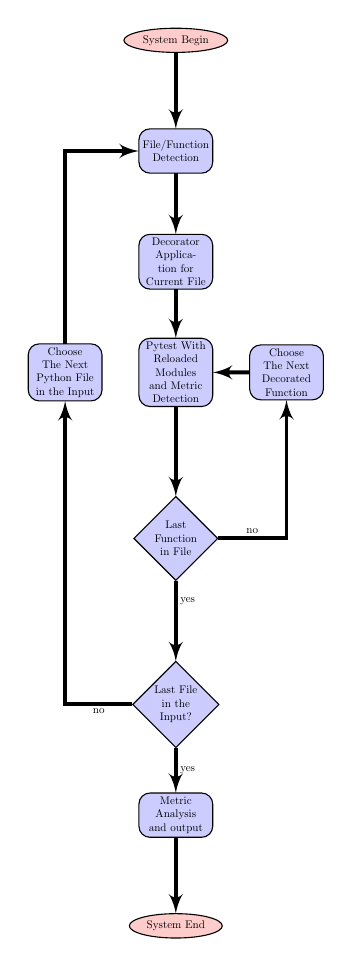
\begin{tikzpicture}[auto, scale=5, every node/.style={scale=0.4}]
    \node [cloud] (sys) {System Begin};
    \node [block, below of=sys, node distance=10em] (file) {File/Function Detection};
    \node [block, below of=file, node distance=10em] (Decorator) {Decorator Application for Current File};
    \node [block, below of=Decorator] (pytest) {Pytest With Reloaded Modules and Metric Detection};
    \node [block, right of=pytest, node distance=10em] (choose) {Choose The Next Decorated Function};
    \node [block, left of=pytest] (Next) {Choose The Next Python File in the Input};
    \node [decision, below of=pytest, node distance=15em] (function) {Last Function in File};
    \node [decision, below of=function, node distance=15em] (Last) {Last File in the Input?};
    \node [block, below of=Last, node distance=10em] (Metric) {Metric Analysis and output};
    \node [cloud, below of=Metric, node distance=10em] (end) {System End};


    \path [line] (sys) -- (file);
    \path [line] (file) -- (Decorator);
    \path [line] (Decorator) -- (pytest);
    \path [line] (pytest) -- (function);
    \path [line] (choose) -- (pytest);
    \path [line] (function) -| node [near start] {no} (choose);
    \path [line] (function) -- node [near start] {yes} (Last);
    \path [line] (Last) -| node [near start] {no} (Next);
    \path [line] (Next) |- (file);
    \path [line] (Last) -- node {yes} (Metric);
    \path [line] (Metric) -- (end);

\end{tikzpicture}

\end{center}


%% Institution logo
\center{

\includegraphics[scale=.95]{img/CollegeLogo}\\
}
}{
%%%%%%%% RIGHT COLUMN
\section{Results}
\begin{table}[H]
\centering

\huge

% \begingroup\small

% \begin{tabular}{rlrrrrrrrrr}
%   \hline

%  & Program & Coverage & Function Cov & NUMM & NUMTM & Fiascoed & Pseudo & NUMTTM & UC & Change \\
%   \hline

%   1 & Hashids-Python & 0.97 & 0.94 &  16 &  15 &  10 &  8 &   7 & 0.44 & 0.50 \\

%   2 & Bleach & 0.48 & 0.41 & 368 & 152 &   8 &   2 & 150 & 0.41 & 0.00 \\

%   3 & Pycco & 0.77 & 0.86 &  22 &  19 &   6 &   5 &  14 & 0.64 & 0.22 \\

%   4 & Howdoi & 0.78 & 0.95 &  20 &  19 &   2 &   0 &  19 & 0.95 & 0.00 \\

%   5 & Flashtext & 0.81 & 0.33 &  42 &  14 &   7 &   4 &  10 & 0.24 & 0.09 \\

%   6 & Honcho & 0.85 & 0.69 &  58 &  40 &   7 &   5 &  35 & 0.60 & 0.09 \\

%   7 & Maya & 0.90 & 0.50 &  88 &  44 &  13 &   3 &  41 & 0.47 & 0.03 \\

%   8 & Gator & 0.99 & 0.86 &  92 &  79 &  54 &  30 &  49 & 0.53 & 0.33 \\

%   9 & Hatch & 1.00 & 0.56 & 134 &  75 &  14 &   6 &  69 & 0.51 & 0.05 \\

%   10 & Nikola & 0.67 & 0.44 & 732 & 319 &  16 &   9 & 310 & 0.42 & 0.02 \\

%    \hline

% \end{tabular}

\begin{tabular}{r|cccc}
  % \hline

  % OLD:
  %  & Program & Coverage & Function Cov & NUMM & NUMTM & Fiascoed & Pseudo & NUMTTM & UC & Change \\
  %  \hline

  Program & Coverage & Total & Modified & Pseudo-Tested \\
  \hline

  % OLD:
  % 1 & Hashids-Python & 0.97 & 0.94 &  16 &  15 &  10 &  8 &   7 & 0.44 & 0.50 \\
  %
  Hashids-Python & 97\% & 16 & 10 & 8 \\

  % 2 & Bleach & 0.48 & 0.41 & 368 & 152 &   8 &   2 & 150 & 0.41 & 0.00 \\

  % 3 & Pycco & 0.77 & 0.86 &  22 &  19 &   6 &   5 &  14 & 0.64 & 0.22 \\

  % 4 & Howdoi & 0.78 & 0.95 &  20 &  19 &   2 &   0 &  19 & 0.95 & 0.00 \\

  % 5 & Flashtext & 0.81 & 0.33 &  42 &  14 &   7 &   4 &  10 & 0.24 & 0.09 \\

  % 6 & Honcho & 0.85 & 0.69 &  58 &  40 &   7 &   5 &  35 & 0.60 & 0.09 \\

  % 7 & Maya & 0.90 & 0.50 &  88 &  44 &  13 &   3 &  41 & 0.47 & 0.03 \\

  % 8 & Gator & 0.99 & 0.86 &  92 &  79 &  54 &  30 &  49 & 0.53 & 0.33 \\

  % 9 & Hatch & 1.00 & 0.56 & 134 &  75 &  14 &   6 &  69 & 0.51 & 0.05 \\

  % 10 & Nikola & 0.67 & 0.44 & 732 & 319 &  16 &   9 & 310 & 0.42 & 0.02 \\

   % \hline

\end{tabular}


% \endgroup



\end{table}


Function-Fiasco can successfully detect pseudo-tested methods in Python based systems.

\section{Future Work}
% Function-Fiasco will be updated to include further return types to fuzz. The purpose is to enhance its ability to detect pseudo-tested methods in systems with varying types of function returns.
Function-Fiasco has many features that will be implemented which include:
\begin{itemize}
  \item{Further type fuzzing capability}
  \item{Parameterized test observation}
  \item{Further system evaluation}
\end{itemize}


\section{Conclusion}
Pseudo-tested methods are an issue that exist in Python based systems. Function-Fiasco has the capability to detect such methods that may lead to unexpected issues. Function-Fiasco can aid in the implementation of Python systems.


\section{Get Involved}
If you would like to get involved, please feel free to enter bugs into the issue tracker on our github page, or submit a pull request to aid in the implementation.
\vfill
% \begin{figure}[b]

\section{Acknowledgements}
Made in cooperation with Cory Wiard.\\


\includegraphics[width=\textwidth]{img/ComputerScience-Stack}
% \end{figure}
}

\end{document}
